\documentclass[]{auvsi_doc}
\setkeys{auvsi_doc.cls}{
	AUVSITitle={UGV Drop Test Description},
	AUVSILogoPath={./figs/logo.pdf},
	AUVSIDocID={GV-007}
}

\usepackage{graphicx}
\usepackage{hyperref}
\hypersetup{
    colorlinks=true,
    linkcolor=blue,
    filecolor=blue,      
    urlcolor=blue,
}
 

\begin{document}
\begin{AUVSITitlePage}
\begin{artifacttable} 
	\entry{GV-008, 1.0, 2-19-2019, Created, Brandon McBride, Jacob Willis}
	\entry{GV-008, 2.0, 03-05-2019, Updated to include predicted landing location, Jacob Willis, Derek Knowles}
\end{artifacttable}
\end{AUVSITitlePage}
% document contents


\section*{Introduction}
This artifact details the methods and results from testing the UGV drop system on the aircraft. 

\section*{Subsystem Test Procedures}
We first started testing the UGV drop with a parachute and a simulated UGV (water bottle with added weight) from the 2nd floor of the Engineering building to the first to see how gently the parachute will cause the UGV to land.
In this test, we already had the parachute deployed and spread out.
Next, we tested dropping the simulated UGV from the top of a 50 foot parking garage. This test showed us that the parachute will deploy in time and reach its terminal velocity.
Once we tested the dropping of the UGV, we began testing the deployment of the UGV from the aircraft.
When we had the bay door built, we set the aircraft on a tall ladder and activated the release mechanism to make sure the parachute wouldn't get caught on the aircraft.
After many successful attempts of deploying the UGV from the aircraft in a controlled environment, we dropped the simulated UGV during a flight test.

\section*{UGV Subsystem Drop Test Result}
A video of the drop test is found in the capstone box folder at: \url{https://byu.box.com/s/wy5dv7jbyjcpto1uvw0xjjnbu4kw6uwq}
The UGV was dropped 120 feet from the ground, about the height we would drop it in the competition. The aircraft was flying at 15 meters per second.
As soon as the UGV was deployed, the dynamics of the aircraft were marginally altered as seen from the slight dip of the aircraft.
The UGV successfully deployed and the landing was gentle. There was a slight drift in the landing as seen from the trail of snow in figure \ref{fig:landing} below.
\begin{figure}[h!]
	\centering
	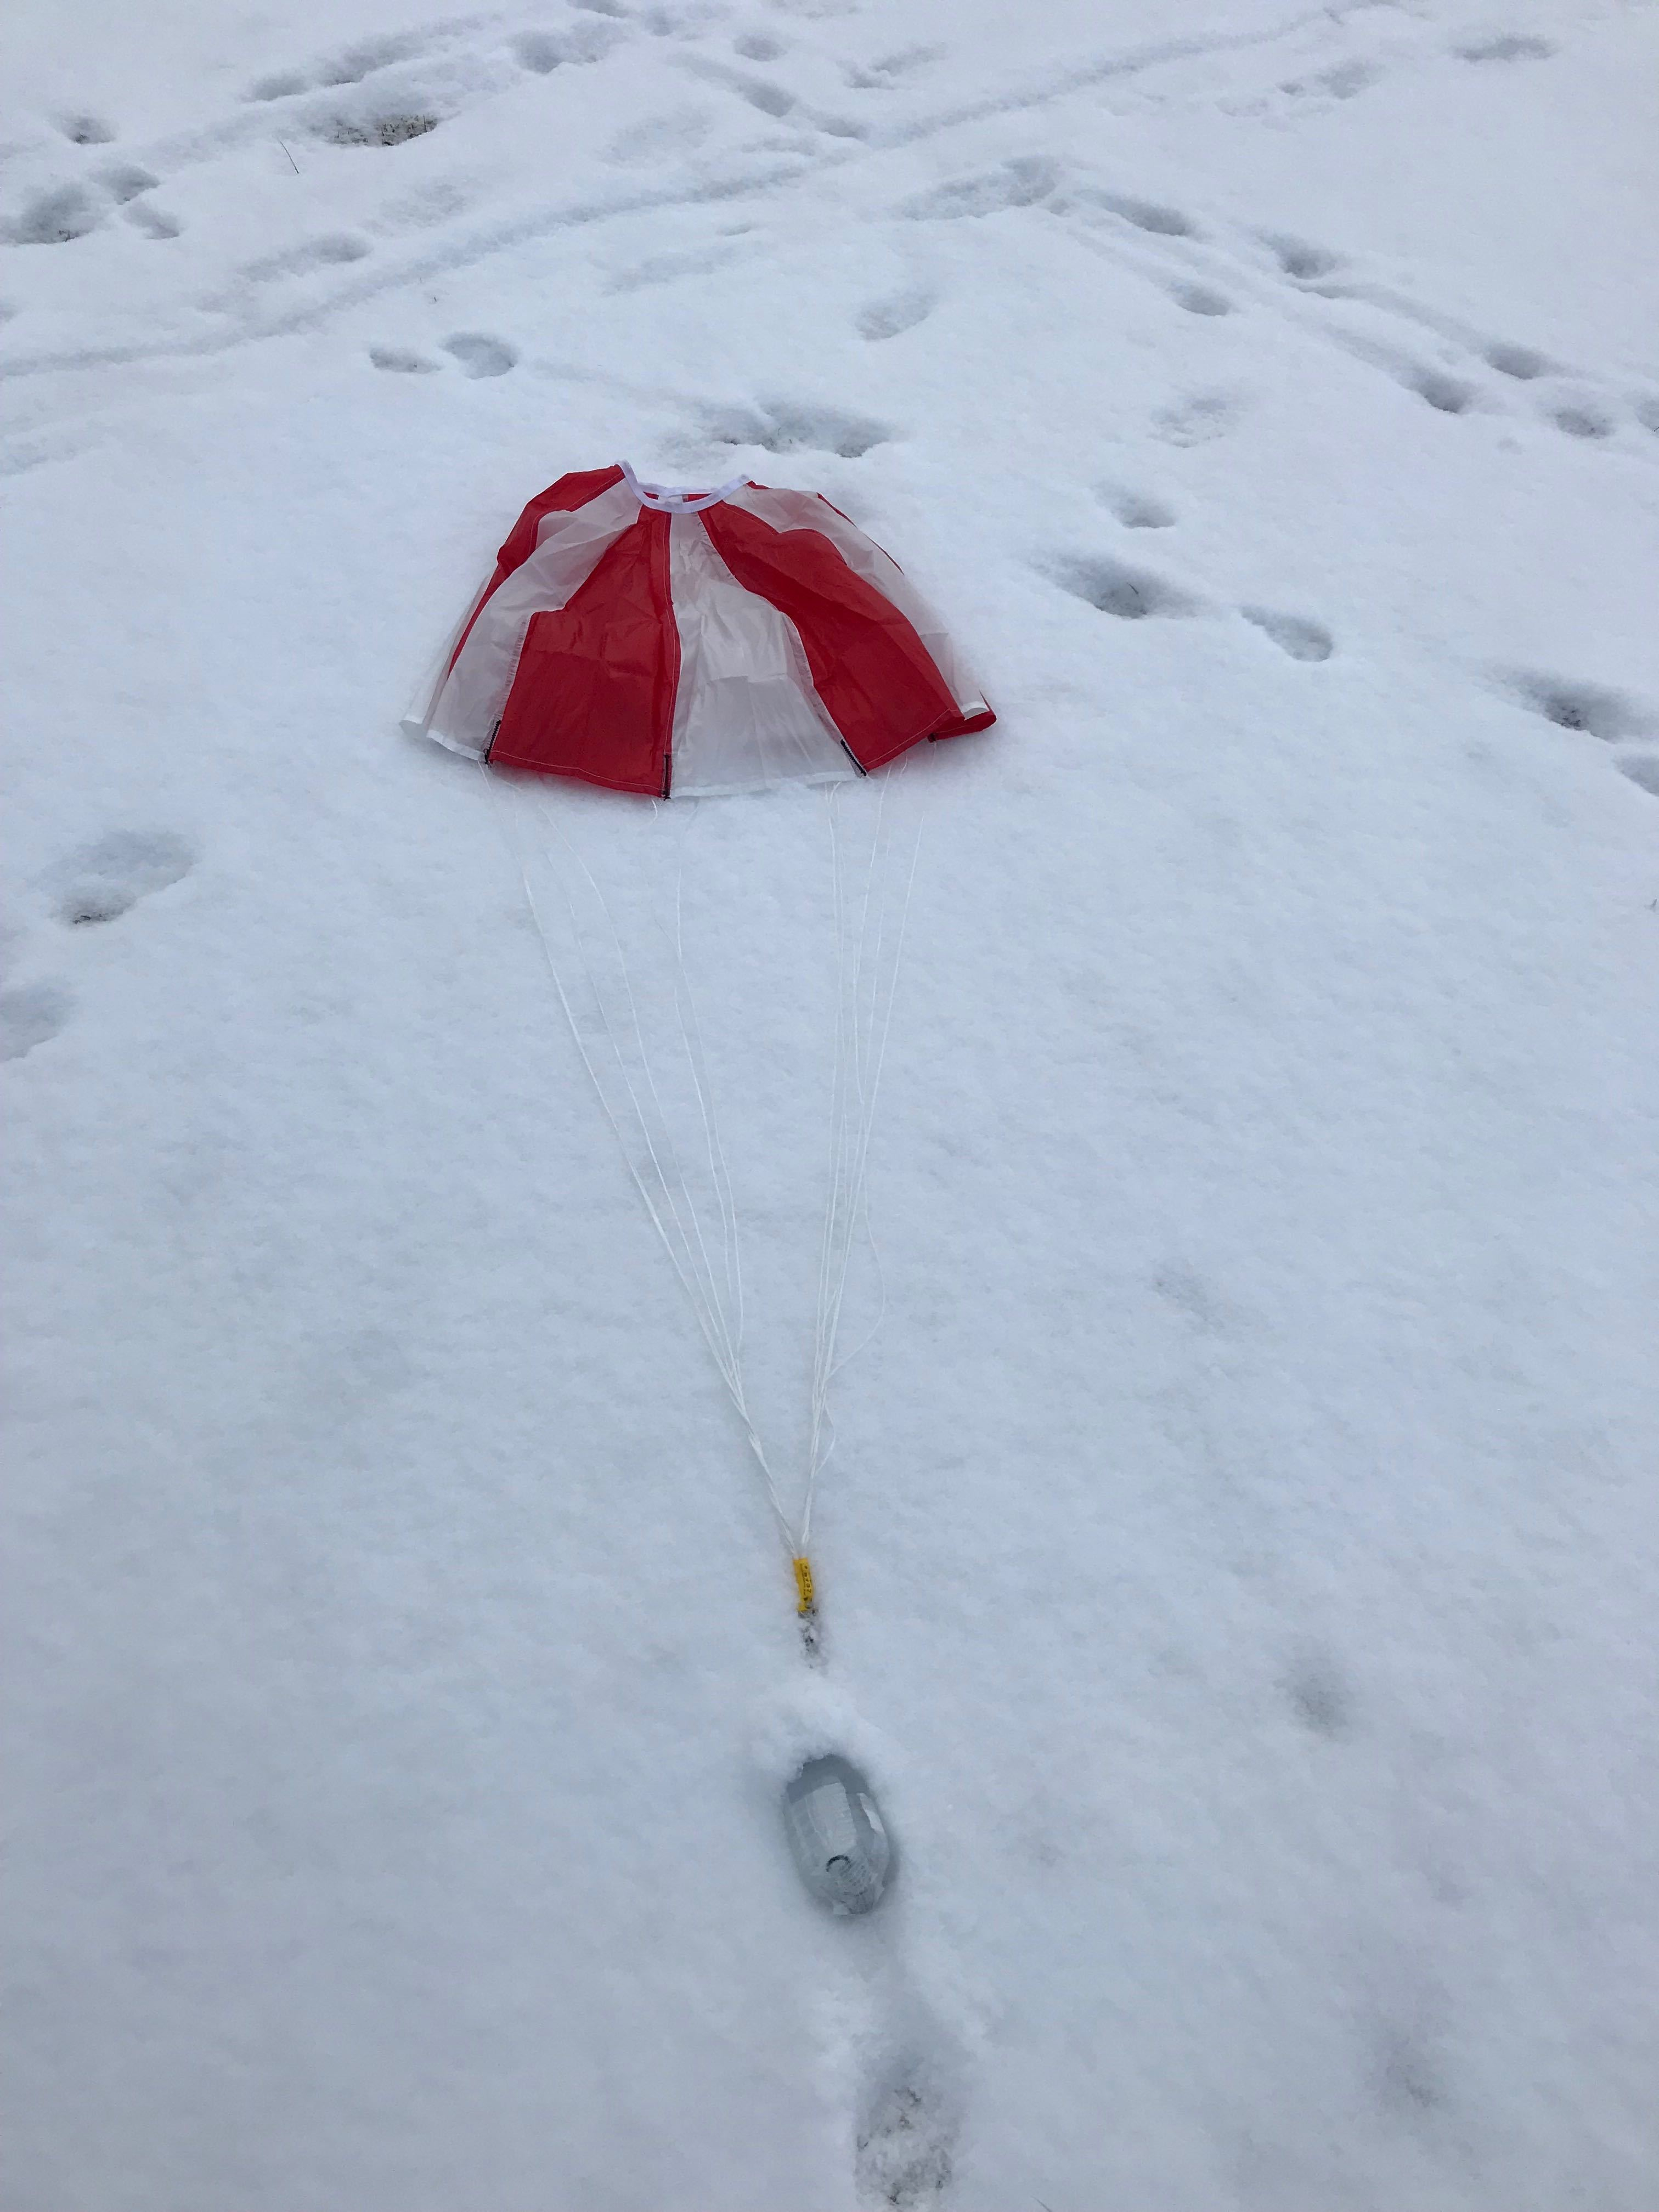
\includegraphics[width=.9\columnwidth]{figs/landing}
	\caption{The snow trail shows movement of the UGV on impact}
	\label{fig:landing}
\end{figure} 


\section*{System Test Procedures}
To test the full UGV drop system, integrated with the UAS autopilot, we used an iPhone with a GPS logger on a mass model of the UGV to measure the path the UGV takes as it is dropped. 
We compared the actual landing location with the location predicted by the UAS.

\section*{UGV System Drop Test Results}
A video of the drop test is found in the capstone box folder at: \url{https://byu.box.com/s/p5om39lsraal1jsgkp95bb4rofm52uic}
In two tests the UGV landed an average distance of 17.7m from the drop location predicted by the UAS.
These tests were performed without an accurate wind estimate on the UAS, so as the wind estimate becomes more accurate, we will be able to improve our drop location.
As it is, the UGV drop subsystem performs within our acceptable range.

\section*{Conclusion}
Our incremental testing of the UGV drop lead to a successful deployment in a flight test, as well as acceptable drop accuracy. Our next step is to work with the autopilot team to improve wind estimation, which will reduce our drop error.

\end{document}
